\documentclass{memo}
\usepackage{graphicx}
\usepackage{hyperref}
\usepackage{listings}
\usepackage{color}

\memoto{Dr. Simoni}
\memofrom{Kyle Daruwalla and Sunil Rao}
\memosubject{Milestone 2 Update}
\memodate{\today}

\definecolor{mygreen}{rgb}{0,0.6,0}
\definecolor{mygray}{rgb}{0.5,0.5,0.5}
\definecolor{mymauve}{rgb}{0.58,0,0.82}

\lstset{ %
  backgroundcolor=\color{white},   % choose the background color; you must add \usepackage{color} or \usepackage{xcolor}
  basicstyle=\footnotesize,        % the size of the fonts that are used for the code
  breakatwhitespace=false,         % sets if automatic breaks should only happen at whitespace
  breaklines=true,                 % sets automatic line breaking
  captionpos=b,                    % sets the caption-position to bottom
  commentstyle=\color{mygreen},    % comment style
  deletekeywords={...},            % if you want to delete keywords from the given language
  escapeinside={\%*}{*)},          % if you want to add LaTeX within your code
  extendedchars=true,              % lets you use non-ASCII characters; for 8-bits encodings only, does not work with UTF-8
  frame=single,                    % adds a frame around the code
  keepspaces=true,                 % keeps spaces in text, useful for keeping indentation of code (possibly needs columns=flexible)
  keywordstyle=\color{blue},       % keyword style
  language=Verilog,                 % the language of the code
  otherkeywords={*,...},            % if you want to add more keywords to the set
  numbers=left,                    % where to put the line-numbers; possible values are (none, left, right)
  numbersep=5pt,                   % how far the line-numbers are from the code
  numberstyle=\tiny\color{mygray}, % the style that is used for the line-numbers
  rulecolor=\color{black},         % if not set, the frame-color may be changed on line-breaks within not-black text (e.g. comments (green here))
  showspaces=false,                % show spaces everywhere adding particular underscores; it overrides 'showstringspaces'
  showstringspaces=false,          % underline spaces within strings only
  showtabs=false,                  % show tabs within strings adding particular underscores
  stepnumber=2,                    % the step between two line-numbers. If it's 1, each line will be numbered
  stringstyle=\color{mymauve},     % string literal style
  tabsize=2,                       % sets default tabsize to 2 spaces
  title=\lstname                   % show the filename of files included with \lstinputlisting; also try caption instead of title
}

\begin{document}

\maketitle

\section{Overview}
For this milestone, we simulated every block down to just above transistor level. The end results were promising, and the simulations in this report document that our FMAC is functioning correctly.

\section{Changes from Initial Design}
All of our changes from the initial design involve the multiplier. We expected that an unsigned multiplier would require sign extension blocks, but this is not the case for a Booth multiplier. The partial products are signed regardless of the input, so we had to implement the correct sign extension blocks. Additionally, we discovered that we needed to use 12-bit adders to allow the sign bits of each partial product to propagate correctly.

\section{Testing}
The code below is our test bench for the FMAC unit.
\begin{lstlisting}
integer i;
initial begin
threshold = 16'd254;
CLK = 1'b0;
RESET = 1'b0;
x = 8'd0;
y = 8'd0;

#20 RESET = 1'b1; y=8'd1;

for (i = 0; i < 8; i = i + 1) begin
    #20 x = 8'd1 << i;
end

#20 x = 8'd1;
for (i = 0; i < 8; i = i + 1) begin
    #20 y = 8'd1 << i;
end

#20 x = 8'd7; threshold = 16'd3565;
for (i = 0; i < 8; i = i + 1) begin
    #20 y = 8'd1 << i;
end

#20 threshold = 16'd65025;
#20 y = 8'b01010101; x = 8'b10101010;
#20 x = 8'hFF; y = 8'hFF;
#40 $finish;

end
always #10 CLK = ~CLK;
\end{lstlisting}

After we verified the test bench with the behavioral model for the FMAC unit, we used the same test bench for the functional model. Using this we verified the functionality for multiplier, accumulator, and comparator within the overall MAC unit. To verify operation we computed powers of two for both x and y inputs into the MAC unit. In addition we verified that the accumulator would be updated on the following positive clock edge. Our reset test cases were with variable threshold values. Our test bench produces sums above the threshold at the end of each subtest. Here we verify the comparator output going low and the accumulator register being appropriately reset to zero. Another test case we used was for when $x = $ 8'b10101010 and $y = $ 8'b01010101 as we believe the product of these two requires many partial products and therefore more addition operations. The final case we tested was the overflow condition. Here we set x and y to be the maximum possible values for 8 bit numbers and verified that when the overall adder overflowed, the accumulator would be reset to zero.

The simulation results for each test case can be found in Figures \ref{fig:testcase1}, \ref{fig:testcase2}, \ref{fig:testcase3}, and \ref{fig:testcase4}. Larger copies of each figure can be found at \url{https://github.com/darsnack/ECE551FMACProject} under the Memos folder.

\begin{figure}[ht]
    \centering
    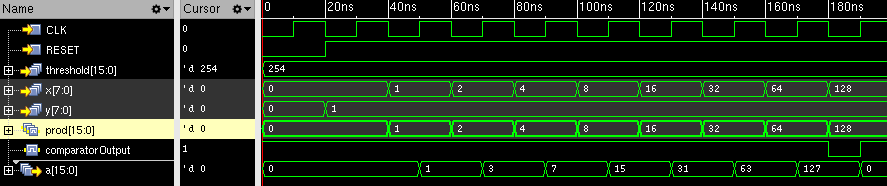
\includegraphics[scale=0.8]{testcase1.png}
    \caption{Testing $y = 1$ and a single bit shifted through $x$}
    \label{fig:testcase1}
\end{figure}
\begin{figure}[ht]
    \centering
    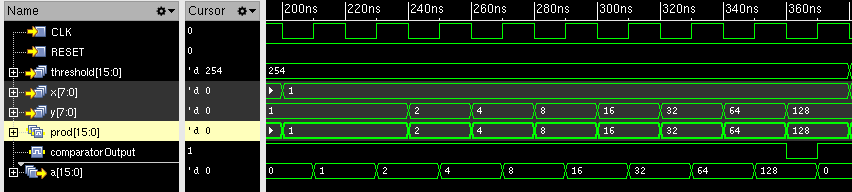
\includegraphics{testcase2.png}
    \caption{Testing $x = 1$ and a single bit shifted through $y$}
    \label{fig:testcase2}
\end{figure}
\begin{figure}[ht]
    \centering
    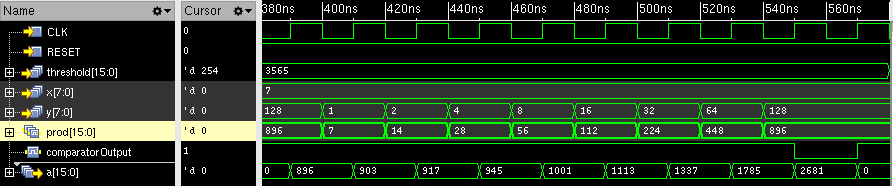
\includegraphics[scale=0.8]{testcase3.png}
    \caption{Testing $x = 7$ and a single bit shifted through $y$}
    \label{fig:testcase3}
\end{figure}
\begin{figure}[ht]
    \centering
    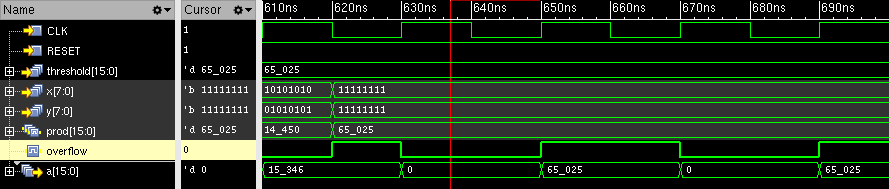
\includegraphics[scale=0.9]{testcase4.png}
    \caption{Testing $x =$ 8'b01010101 and $y =$ 8'b10101010}
    \label{fig:testcase4}
\end{figure}

\newpage
\section{Code}
We have included some of the complex Verilog code. We elected not to include the adder and comparator, because their design is standard above transistor level. All code can be found at \url{https://github.com/darsnack/ECE551FMACProject} under the Verilog folder.

Below is the functional view for the FMAC unit. The multiplier and full adder have functional views that are broken down into smaller functional views. The comparator is left behavioral as the next step down is the transistor design.
\begin{lstlisting}
module fmac(input CLK, input RESET, input [7:0] x, input [7:0] y,
            input [15:0] threshold, output reg [15:0] a);

reg [15:0] accumulator;
wire [15:0] prod;
wire [15:0] sum;
wire comparatorOutput;
wire overflow;

initial begin
    a = 16'd0;
    accumulator = 16'd0;
end

multiplier multiplier(
    .x(x),
    .y(y),
    .multOut(prod));
fadder adder(
    .a(accumulator),
    .b(prod),
    .s(sum),
    .co(overflow));
comparator comparator(
    .CLK(CLK),
    .a(sum),
    .b(threshold),
    .result(comparatorOutput));

always @(posedge CLK) begin
    if (RESET == 0) begin
        a <= 16'd0;
        accumulator <= 16'd0;
    end if ((~comparatorOutput)||overflow) begin
        a <= 16'd0;
        accumulator <= 16'd0;
    end else begin
        a <= sum;
        accumulator <= sum;
    end
end


endmodule
\end{lstlisting}

Below is the functional view for the multiplier unit. Here the Booth encoder and decoder are broken down into functional views to the smallest 3-bit encoding views. The adder is broken down into 1-bit adders and the sign extender is already 1 level above transistors.
\begin{lstlisting}
module multiplier(input [7:0] x, input [7:0] y, output [15:0] multOut);
    //encoder outputs
    wire [2:0] a0;
    wire [2:0] a1;
    wire [2:0] a2;
    wire [2:0] a3;
    wire [2:0] a4;
    //partial product outputs
    wire [9:0] pp0;
    wire [9:0] pp1;
    wire [9:0] pp2;
    wire [9:0] pp3;
    wire [9:0] pp4;
    //sign extended partial products
    wire [9:0] extendedpp0;
    wire [9:0] extendedpp1;
    wire [9:0] extendedpp2;
    wire [9:0] extendedpp3;
    wire [9:0] extendedpp4;
    //addition outputs
    wire cout0, cout1, cout2,cout3;
    wire [12:0] s0;
    wire [12:0] s1;
    wire [12:0] s2;
    wire [12:0] s3;

    BoothEncoder8bit encode(.x(x),.a0(a0),.a1(a1),.a2(a2),.a3(a3),.a4(a4));
    BoothDecoder8bit decode(.y(y),.a0(a0),.a1(a1),.a2(a2),.a3(a3),.a4(a4),
                            .pp0(pp0),.pp1(pp1),.pp2(pp2),.pp3(pp3),.pp4(pp4));

    SignExtender partial0(.partialProduct(pp0),.ppNum(1'b1),.extendedPartialProduct(extendedpp0));
    SignExtender partial1(.partialProduct(pp1),.ppNum(1'b0),.extendedPartialProduct(extendedpp1));
    SignExtender partial2(.partialProduct(pp2),.ppNum(1'b0),.extendedPartialProduct(extendedpp2));
    SignExtender partial3(.partialProduct(pp3),.ppNum(1'b0),.extendedPartialProduct(extendedpp3));
    SignExtender partial4(.partialProduct(pp4),.ppNum(1'b0),.extendedPartialProduct(extendedpp4));

    adder10bit adder0(.a({3'b001, extendedpp1}),.b({3'd0, extendedpp0}),.cin(1'b0),.cout(cout0),.s(s0));
    adder10bit adder1(.a({3'b001, extendedpp2}),.b({2'd0, s0[12:2]}),.cin(cout0),.cout(cout1),.s(s1));
    adder10bit adder2(.a({3'b001, extendedpp3}),.b({2'd0, s1[12:2]}),.cin(cout1),.cout(cout2),.s(s2));
    adder10bit adder3(.a({3'b000, extendedpp4}),.b({2'd0, s2[12:2]}),.cin(cout2),.cout(cout3),.s(s3));

    assign multOut = {s3[7:0],s2[1:0],s1[1:0],s0[1:0],pp0[1:0]};

endmodule
\end{lstlisting}

\end{document}